\documentclass[ignorenonframetext]{beamer}
\usetheme{metropolis}
\usepackage{amssymb,amsmath}
\definecolor{links}{HTML}{2A1B81}
\hypersetup{colorlinks,linkcolor=,urlcolor=links}
\usepackage[T1]{fontenc}
\usepackage[utf8]{inputenc}
\usepackage{microtype}
\usepackage{longtable, booktabs}
\usepackage[english]{babel}
\usepackage{pgf, microtype, booktabs, times, etex}
\usepackage{tcolorbox}
\tcbuselibrary{minted,skins}

\newtcblisting{latexcode}{
	listing engine=minted,
	colback=bashcodebg,
	colframe=black!70,
	listing only,
	minted style=colorful,
	minted language=latex,
	minted options={linenos=true,texcl=true},
	left=1mm,
}
\definecolor{bashcodebg}{rgb}{0.85,0.85,0.85}
%\usemintedstyle{emacs}
\beamertemplatenavigationsymbolsempty

\title{\LaTeX{} for Economics and Business Administration}
\author{Thomas de Graaff}
\date{January 13, 2020}

\titlegraphic{%
  \vspace{4.2cm}\flushright\ 
\includegraphics[width = 0.3\textwidth]{cookies} }

\begin{document}
\frame{\titlepage}

\section{Introduction}\label{introduction}

\begin{frame}{Why this workshop?}

\begin{itemize}
\item
  In the \alert{social sciences} few attention to what tools to use (and why)
    \begin{itemize}
      \item you just use what colleagues, friends or teachers used
      \item huge fixed (and sometimes sunk) costs \newline \pause
    \end{itemize}
\item
  Increasing use of \LaTeX{}
  \begin{itemize}
    \item more user friendly (editors, online environments)
    \item combination with markdown used on internet/blogs
    \item tight connection with (statistical) software (\texttt{R}/\texttt{Python}/\texttt{Stata})
    \item combination with \alert{data science}
  \end{itemize}
\end{itemize}
\end{frame}

\begin{frame}{What I want (and don't want) with this workshop}

\begin{itemize}
\item
  Give a general introduction of why some tools work together

  \begin{itemize}
  \item \LaTeX{}
  \item reference managers
  \item (statistical) output
  \end{itemize}
\item
  Give an introduction to \LaTeX{}

  \begin{itemize}
	  \item First \alert{vanilla basics} (including references)
	  \item Next workshop: more advanced stuff
  \end{itemize}
\item
  What \emph{I} do not want

  \begin{itemize}
  \item
    Tell you what applications to use (\alert{you} need to decide and make a \alert{well-informed} decision)
  \end{itemize}
\end{itemize}

\end{frame}

\begin{frame}[fragile]{Background}

  \begin{columns}
    \begin{column}{.5\textwidth}
      \begin{itemize}
        \item \TeX{} created by Donald Knuth (70's)
        \item \LaTeX{} is a set of macro's around TeX (1986)
        \item \LaTeX{} is a \alert{typesetting program}, not a \alert{Word
          processor}
          \begin{itemize}
            \item So \alert{edit} code that needs to be compiled
          \end{itemize}
          \begin{itemize}
            \item Editors
              \begin{itemize}
                \item specific: TeXstudio, TeXshop, Rstudio
                \item general: Sublime, Atom, Vim, Emacs
              \end{itemize}
          \end{itemize}
        \end{itemize}
    \end{column}

    \begin{column}{.5\textwidth}
      \begin{figure}[h]
        \centering
        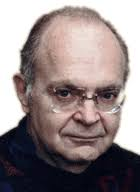
\includegraphics[width = 0.7\textwidth]{knuth}
        \newline
        \begin{footnotesize}
        ``Beware of bugs in the above code; I have only proved it correct, not tried it.''
        \end{footnotesize}
        \end{figure}
    \end{column}
  \end{columns}
\end{frame}

\begin{frame}[fragile]
  \frametitle{Showcase: Tufte lay-out style}
  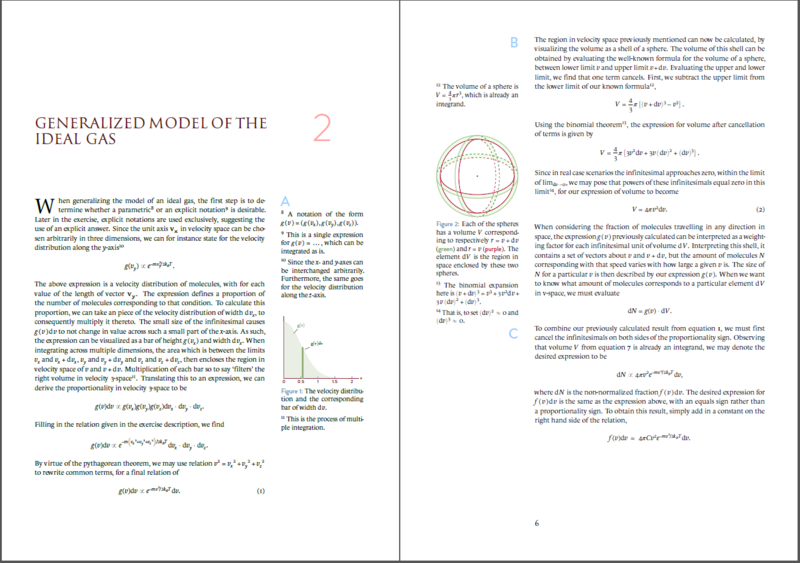
\includegraphics[width = 1.0\textwidth]{tufte}
\end{frame}

\begin{frame}[fragile]
  \frametitle{Showcase: tikz and PGFPlots}
  \begin{columns}
    \begin{column}{.5\textwidth}

  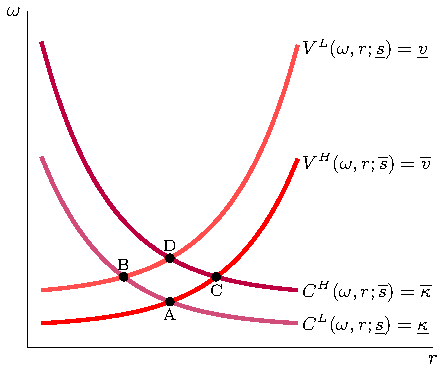
\includegraphics[width = 1.0\textwidth]{CostUtility}
    \end{column}

    \begin{column}{.5\textwidth}

  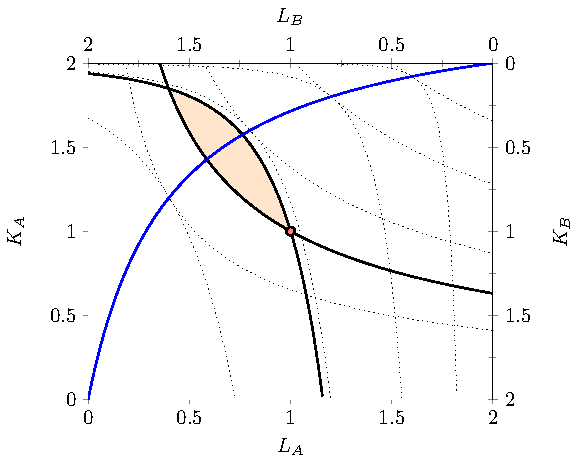
\includegraphics[width = 1.0\textwidth]{vraag1e}
    \end{column}
  \end{columns}
\end{frame}

\begin{frame}[fragile]
  \frametitle{Showcase: posters}
  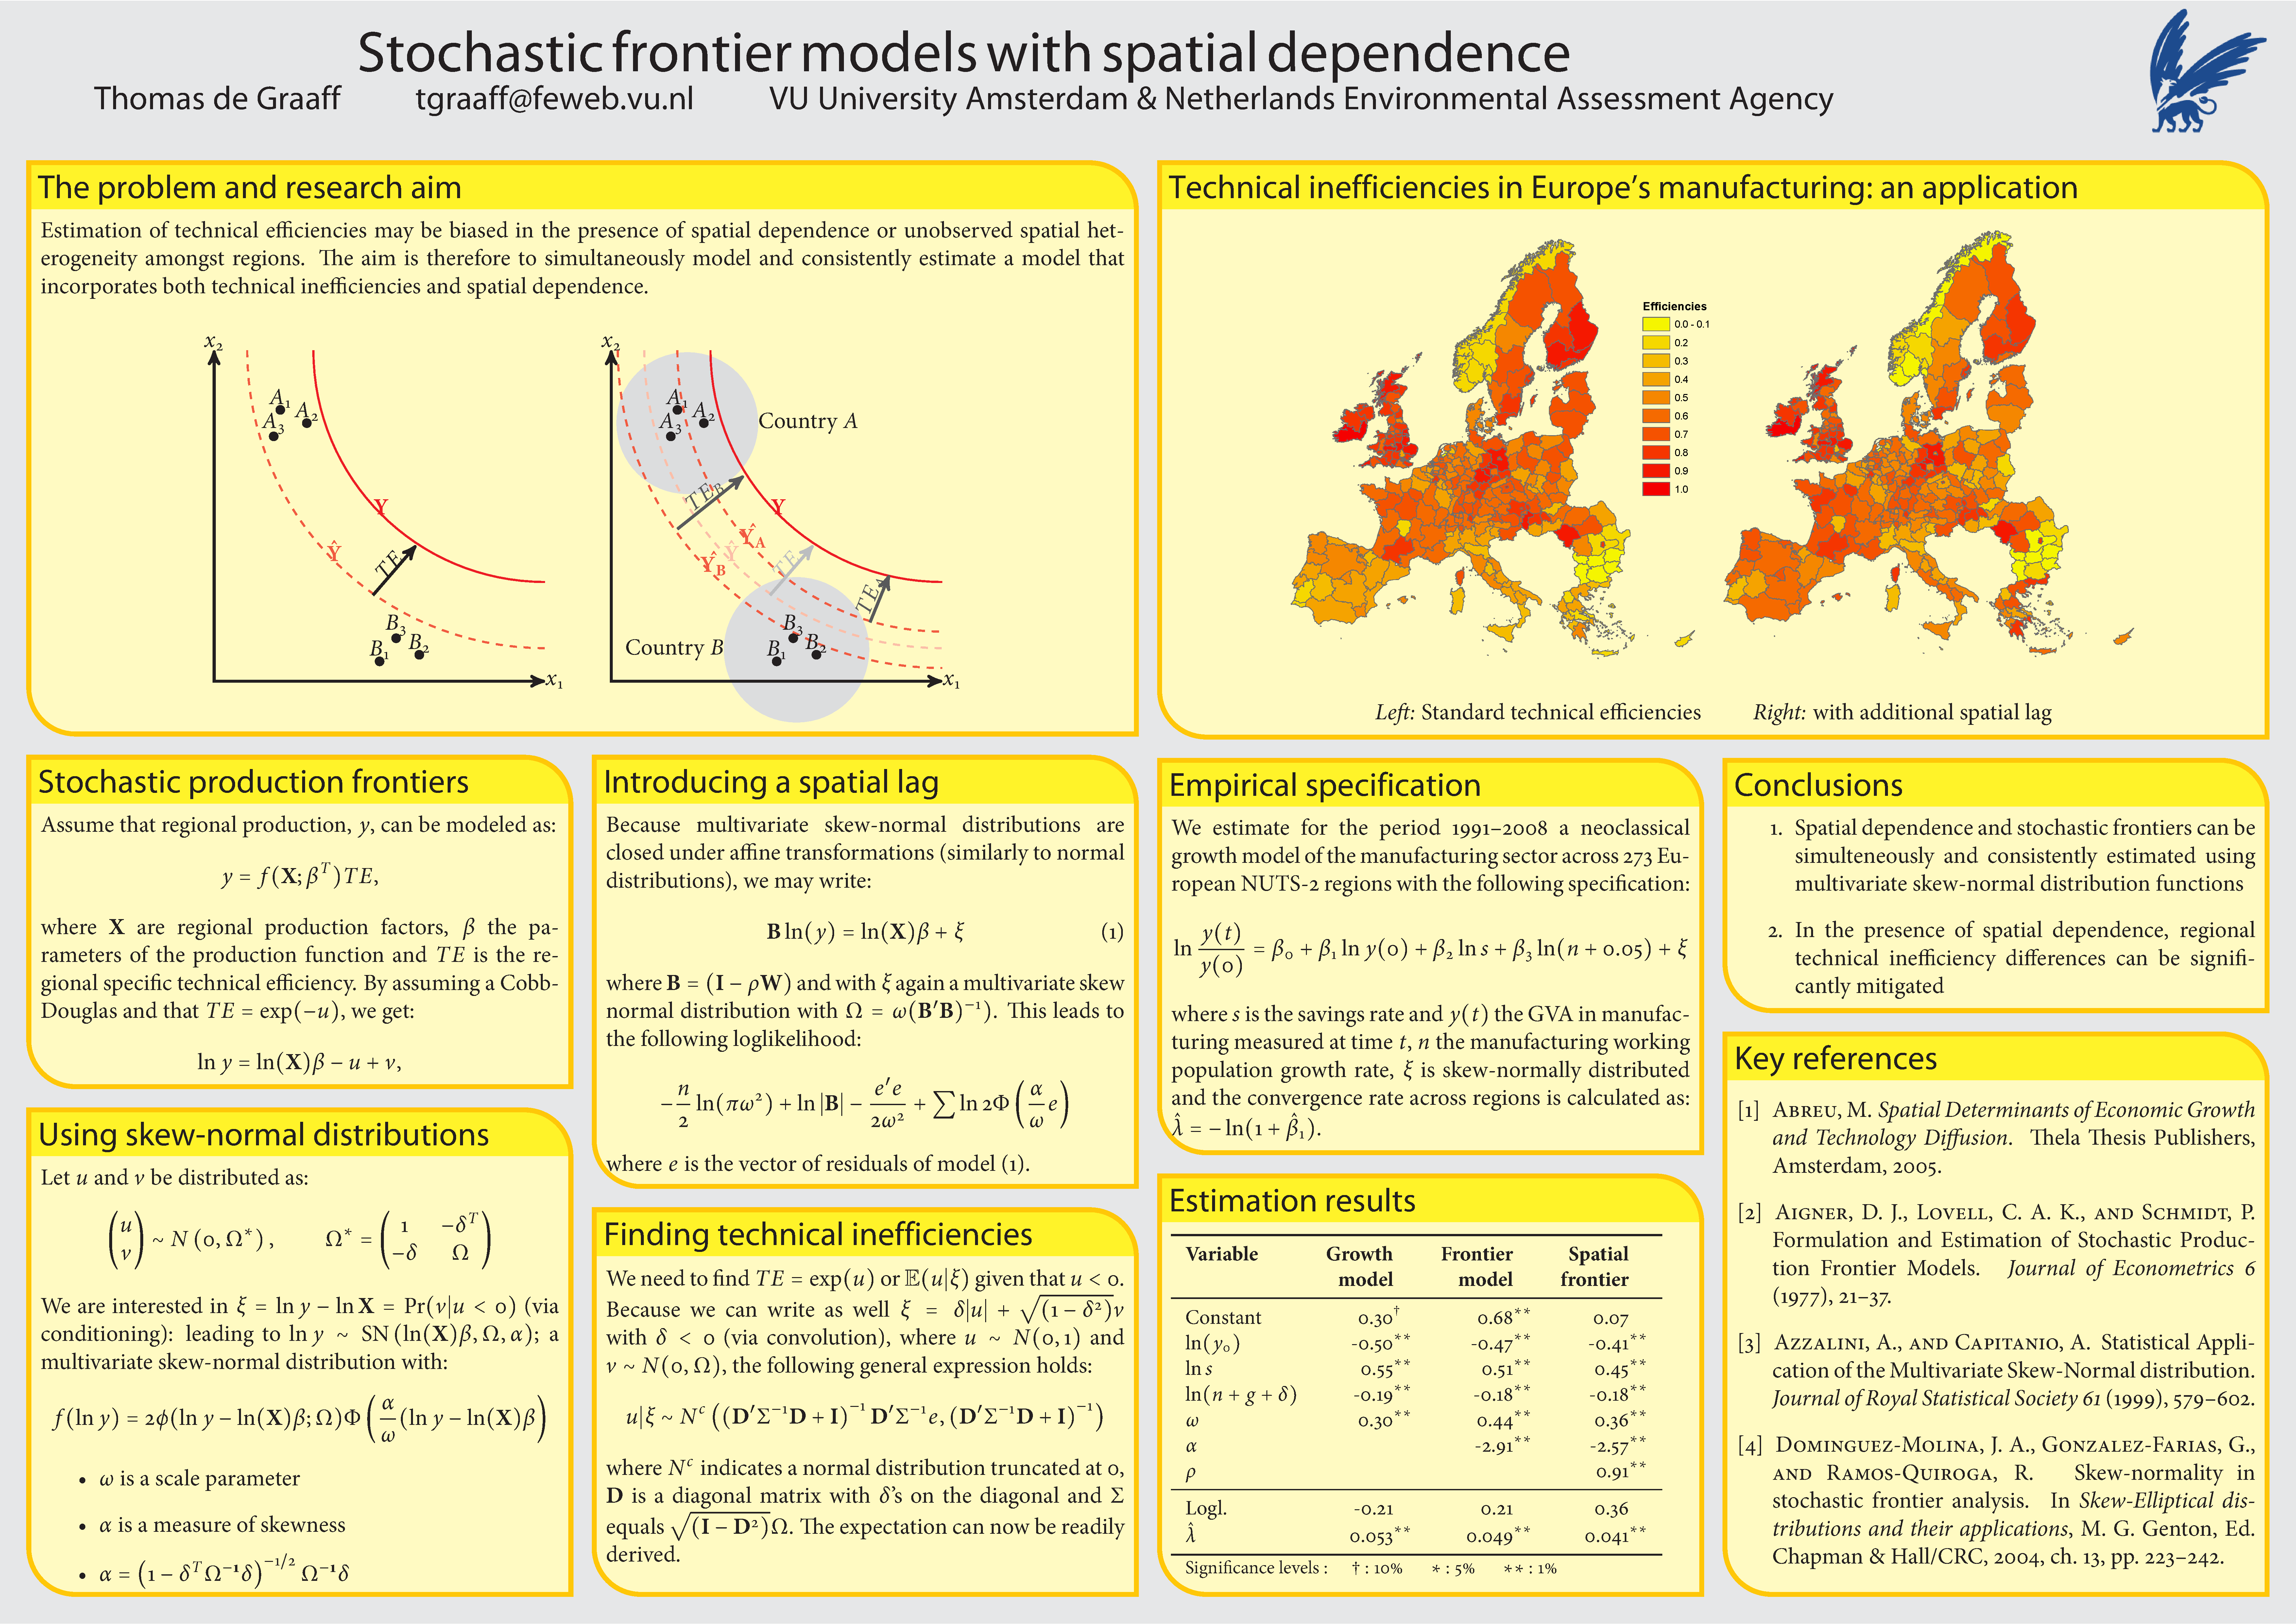
\includegraphics[width = 1.0\textwidth]{poster}
\end{frame}

\subsection{Why \LaTeX{}?}\label{why}

\begin{frame}{Disadvantages}

\begin{itemize}
  \item not WYSIWYG \pause
  \item you nead to learn (quite) some commands
  \begin{itemize}
  \item
    Learning curve, but
  \item
    hurray for
    \href{https://wch.github.io/latexsheet/latexsheet.pdf}{cheat sheets}
    and Google\pause
  \end{itemize}
  \item Difficult to cooperate with people from the \alert{other} side \pause
\item
  \alert{Basic} \LaTeX{} has difficulties with incorporating new
  fonts (Hoefler, minion pro)
  \begin{itemize}
    \item XeTeX \item For the purists: \LaTeX{} does it right
      \href{http://oestrem.com/thingstwice/2007/05/latex-vs-word-vs-writer/}{(\LaTeX{}
      vs Word)}\pause
  \end{itemize}
  \item Difficult to create unstructured and ugly documents
\end{itemize}
\end{frame}

\begin{frame}{Advantages}

\begin{itemize}
  \item free (as in beer \& in speach)\pause
  \item WYSIWYM \pause
  \item consistent lay-out throughout the whole document (including tables,
    appendices, formulas, source code, etc) \pause
  \item internal references are a breeze (citations, ToC, ToT \ldots{})\pause
  \item forced to structure documents\pause
  \item macros around plain text, thus scriptable\pause
  \item large community, thus a package for almost everything (books, articles,
    presentation, posters, exams, musicscores)\pause
  \item superior typography \& output \pause
  \item many free
    \href{https://www.overleaf.com/latex/templates/}{\LaTeX~templates}
\end{itemize}

\end{frame}

\begin{frame}{\LaTeX{} versus Markdown}
	\begin{itemize}
		\item
    \href{https://www.overleaf.com/learn/latex/Articles/How_to_write_in_Markdown_on_Overleaf}{markdown}:
    \begin{itemize}
      \item
    lightweight markup language that can export
      to \texttt{.doc}, \texttt{.html}, and \texttt{.pdf}. \newline
    \end{itemize}
		\item much easier then \LaTeX{} but less flexible \newline
		\item used by writers/blogs even for complete websites \newline
		\item interaction with \LaTeX{}; if not only for formula's
	\end{itemize}
\end{frame}

\begin{frame}[fragile]
  \frametitle{Some thoughts on overleaf}
  \begin{columns}
    \begin{column}{.5\textwidth}
      \alert{pro}
      \begin{itemize}
        \item great learning environment
        \item track changes
        \item rich text
        \item cooperation
        \item great documentation\pause
      \end{itemize}
    \end{column}
    \begin{column}{.5\textwidth}
      \vspace*{0cm}
      \alert{con}

      \begin{itemize}
        \item you need to be online
        \item proprietary software
        \item standalone
        \item backing-up
      \end{itemize}
    \end{column}
  \end{columns}

\end{frame}

\subsection{Technicalities}\label{technicalities}

\begin{frame}[fragile]{How does \LaTeX{} work in practice?}

\begin{itemize}
\item
  You edit a \texttt{.tex} file without thinking about how it looks

  \begin{itemize}
  \item
    distraction free writing (yeah right)
    \newline
  \end{itemize}
\item
  You then compile it

  \begin{itemize}
  \item
    \LaTeX{} is unforgiving: if there is an error, usually it does not
    compile
  \item
    Typically, errors are missing brackets or parentheses.\newline
  \end{itemize}
\item
  Typically, source \texttt{.tex} file is compiled into \texttt{.pdf}
\end{itemize}
\end{frame}


\section{TeXstudio}

\subsection{How to work with TeXstudio}

\begin{frame}{TeXstudio: A quick tour}
	\begin{itemize}
		\item Preferences \newline
		\item Keyboard shortcuts \newline
		\item LaTeX dropdown menu
	\end{itemize}
\end{frame}

\section{Exercises}

\subsection{Baby-steps}

\begin{frame}{First: organize!}
	\begin{enumerate}
		\item Create a specific workshop folder somewhere where you can find it.
		\newline
		\item Think about versioning system and a back-up system
		\newline
		\item E.g.: use dropbox and/or Time Machine 
	\end{enumerate}
\end{frame}

\begin{frame}[fragile]{Exercise 1: Open from template and fill in!}
\small
\begin{latexcode}
\documentclass[]{article}
%opening
\title{}
\author{}

\begin{document}
	
\maketitle

\begin{abstract}
	
\end{abstract}

\section{}
	
\end{document}
\end{latexcode}
\end{frame}

\begin{frame}{OK; and now what?}
	\begin{enumerate}
		\item Save your file in your folder (give it an appropriate name)
		\newline
		\item Press \texttt{F1} (or \texttt{F5})
		\newline
		\item The editor now sends \LaTeX{} the message that it should \textit{compile} your file
		\newline
		\item \LaTeX{} creates many new files
	\end{enumerate}
\end{frame}

\subsection{Paper structure}

\begin{frame}[fragile]{Exercise 2: Create a paper structure}
	\small
	\begin{latexcode}
\section{}
\subsection{}
\subsubsection{}
	\end{latexcode}
Note that the following are used for books
\small
\begin{latexcode}
\part{}
\chapter{}
\end{latexcode}
And for bigger projects:
\begin{latexcode}
\include{}
\input{}
\end{latexcode}
\end{frame}

\begin{frame}[fragile]{Intermezzo: preamble}
Part before \texttt{\textbackslash begin document} is called preamble
\begin{latexcode}
\documentclass[]{article}

% This is where packages are loaded 
% and specific commands are given that 
% determine how the lay-out and desing
% of your document will look like 
% including: references, tables, 
% paragraphs, headers, etc.
	
\begin{document}
\end{latexcode}	
\end{frame}

\begin{frame}[fragile]{Intermezzo: white spaces and special characters}
An empty line starts a new paragraph and consecutive white spaces are treated as one
\begin{latexcode}
One paragraph

Second     paragraph (just one white space)
\end{latexcode}	

The following characters are reserved \# \$ \% \^ \& \_ \{ \} \~{} \textbackslash{} and should be used as follows
\begin{latexcode}
  \# \$ \% \^ \& \_ \{ \} \~ \\
\end{latexcode}
So, with a backslash before except for the backslash (does this make sense?)
\end{frame}

\begin{frame}[fragile]{Exercise 3: Create a table of contents}
More complex text structures are relatively easy, just insert (after \texttt{\textbackslash begin document})
\begin{latexcode}
\tableofcontents
\listoffigures
\listoftables
\end{latexcode}
\end{frame}

\begin{frame}[fragile]{Lists}
\begin{itemize}
	\item Itemization
\begin{latexcode}
\begin{itemize}
	\item blue
	\item red
\end{itemize}
\end{latexcode}	
	\item Enumeration
\begin{latexcode}
\begin{enumerate}
	\item first item
	\item second item
\end{enumerate}
\end{latexcode}	
\end{itemize}
\end{frame}

\begin{frame}[fragile]{Exercise 4: Lists}
	Create the following mode choice list in your \texttt{.tex} document\\
	\\
	\begin{enumerate}
		\item Cycling
		\item Walking
		\item Driving
		\item Public transport
		\begin{itemize}
			\item Bus
			\item Tram
			\item Metro
			\item Train
		\end{itemize} 
	\end{enumerate}
\end{frame}

\begin{frame}[fragile]{Further text control}
\begin{itemize}
\item Bold
\begin{latexcode}
\textbf{bold}
\end{latexcode}		
\item Emphasize
\begin{latexcode}
\textit{italics} or \emph{emphasized}
\end{latexcode}		
\end{itemize}
\end{frame}

\subsection{Formula's} 

\begin{frame}[fragile]{Formula's}
Inline math \texttt{\$ \$}; displayed math \texttt{\$\$ \$\$}; for example:
\begin{latexcode}
$x^2$
$x_2$
$\sqrt{x}$
$$Y = K^\alpha L^{1-\alpha}$$
$$\sum_{i=1}^I$$
$$\frac{\partial x}{\partial y}$$
\begin{equation}
	E = mc^2
\end{equation}
\end{latexcode}
\end{frame}

\begin{frame}{Exercise 5: Create these formula's}
	\begin{enumerate} 
		\item Regression formula:
		\[ y_i = \alpha + \beta x_i + \epsilon_i \]
		\item The mean
		$$\bar{x} = \frac{1}{N}\sum_{i=1}^N x_i$$
		\item Optimal economic order quantity:
		$$Q^\ast = \sqrt{ \frac{2DK}{h}} $$
	\end{enumerate}
\end{frame}

\subsection{Figures}

\begin{frame}[fragile]{Figures}
	Figures/graphs and tables in a floating environment\\
\begin{latexcode}
\begin{figure}[h!]}
\center
	
\includegraphics{ligatures_latex}
	\caption{A figures about ligatures}
	\label{fig:ligatures}
\end{figure}
\end{latexcode}
Figures can be \texttt{.pdf}, \texttt{.jpg}, \texttt{.png} and a whole lot of other types (but not bitmaps!)
\end{frame}

\subsection{Tables}

\begin{frame}[fragile]{Tables}
\begin{latexcode}
\begin{table}[t!]
	\caption{This is the caption}
	\begin{tabular}{|l|c|r|}
		\hline
		first & row & data \\
		second & row & data \\
		\hline
	\end{tabular}
	\label{tab:example}
\end{table}
\end{latexcode}
\end{frame}

\subsection{Referencing}

\begin{frame}[fragile]{Referencing}
Internal references are a breeze
\begin{latexcode}
\label{}	% Label something
\ref{}	% Refer to that
\footnote{}	% Add footnote
\thanks{}	% For in title
\end{latexcode}
\end{frame}

\begin{frame}[fragile]{Exercise 6: Create a table}
Create the following table 

\begin{table}[!th]
	\center
	\caption{Average grades}
	\begin{tabular}{lrr}
		\hline
		First name  & Surname & Grade \\
		\hline
		Sherlock & Holmes & 7.9 \\
		John H. & Watson & 8.1 \\
		\hline
		\\
		\\
	\end{tabular}
	\label{tab:grades}
\end{table}

And refer to it in text as such: 
\begin{quote}
	Table \ref{tab:grades} gives the average grades for course \textit{solving crimes}.
\end{quote}
\end{frame}

\begin{frame}[fragile]{BibTeX}
Literature references (at the end)
\begin{latexcode}
\cite{} % cite something
% Now tell LaTeX where to find references	
\bibliography{references.bib}
% and which citation style to use
\bibliographystyle{apalike}
\end{latexcode}
Later, we dive into how to make this look good
\end{frame}

\begin{frame}{Exercise 7: References}
	\begin{enumerate}
		\item Search on Google Scholar for three references from Erik Verhoef and/or Wout Dullaert
		\newline
		\item Put those in a \texttt{.bib} file in the \textbf{same} directory as your \texttt{.tex} file
		\newline
		\item Refer to those in your \texttt{.tex} file
		\newline
		\item Create the reference list
	\end{enumerate}
\end{frame}

\section{Conclusion}

\subsection{Next time}

\begin{frame}{Next workshop}
	\begin{itemize}
		\item Use of packages
		\newline
		\item Making things look better!
		\newline
		\item Graphs
		\newline
		\item Better tables with \texttt{Stata} and \texttt{R} output
		\newline
		\item Slides
	\end{itemize}
\end{frame}

\end{document}

%%% Local Variables:
%%% LaTeX-command: "latex -shell-escape"
%%% End:
